%
% Complete documentation on the extended LaTeX markup used for Insight
% documentation is available in ``Documenting Insight'', which is part
% of the standard documentation for Insight.  It may be found online
% at:
%
%     http://www.itk.org/

\documentclass{InsightArticle}


%%%%%%%%%%%%%%%%%%%%%%%%%%%%%%%%%%%%%%%%%%%%%%%%%%%%%%%%%%%%%%%%%%
%
%  hyperref should be the last package to be loaded.
%
%%%%%%%%%%%%%%%%%%%%%%%%%%%%%%%%%%%%%%%%%%%%%%%%%%%%%%%%%%%%%%%%%%
\usepackage[dvips,
bookmarks,
bookmarksopen,
backref,
colorlinks,linkcolor={blue},citecolor={blue},urlcolor={blue},
]{hyperref}
% to be able to use options in graphics
\usepackage{graphicx}
% for pseudo code
\usepackage{listings}
% subfigures
\usepackage{subfigure}


%  This is a template for Papers to the Insight Journal.
%  It is comparable to a technical report format.

% The title should be descriptive enough for people to be able to find
% the relevant document.
\title{WrapITK: Enhanced languages support\\ for the Insight Toolkit}

% Increment the release number whenever significant changes are made.
% The author and/or editor can define 'significant' however they like.
\release{0.2.2}

% At minimum, give your name and an email address.  You can include a
% snail-mail address if you like.
\author{Ga\"etan Lehmann{$^1$}{\small{,}} Zachary Pincus{$^2$} {\small{and}} Benoit Regrain{$^3$}}
\authoraddress{{$^1$}INRA, UMR 1198; ENVA; CNRS, FRE 2857, Biologie du D\'eveloppement et
Reproduction, Jouy en Josas, F-78350, France\\
{$^2$}Program in Biomedical Informatics and Department of Biochemistry, Stanford University School of Medicine, Stanford, California\\
{$^3$}CREATIS, CNRS UMR 5515, Inserm U630, Univ. Lyon1, INSA Lyon, 69621 Villeurbanne, France}

\begin{document}
\lstset{language=python}
\maketitle

\ifhtml
\chapter*{Front Matter\label{front}}
\fi

\begin{abstract}
\noindent
ITK \cite{ITKWebSite} is a huge image analysis library, which contains lots of state of the art
algorithms implementations. However, using it in C++ can be difficult and is
poorly suited for prototyping. WrapITK aims to allow classes from ITK
(and custom, classes that interact with ITK) to be "wrapped" for use with
languages like Python \cite{PythonWebSite}, Tcl \cite{TclWebSite}, and Java \cite{JavaWebSite}.
\end{abstract}

\tableofcontents

\newpage
\part{Introduction}

WrapITK is a project designed to allow classes from ITK (and custom classes
that interact with ITK) to be "wrapped" for use with languages like
Python \cite{PythonWebSite}, Tcl \cite{TclWebSite}, and Java \cite{JavaWebSite}.

Note that ITK already has a wrapping infrastructure, and that WrapITK is based
on it, and use the same tools: CMake \cite{CMakeWebSite}, GCC-XML \cite{GccxmlWebsite}
and CableSwig\footnote{CableSwig is based on a now quite old version of SWIG
\cite{SwigWebSite}.} \cite{CableSwigWebSite}. This project aims to
address the following deficits of the existing wrappers (and others):
\begin{itemize}
  \item  ITK is a huge library, but only a small number of classes are available
in target languages. This quickly becomes frustrating for the user, especially when
he has to spend lot of time to extend the current set of classes. Even if it is
not yet complete, the WrapITK's set of classes have been highly extended. Moreover,
the user can choose at build time which types and which dimensions he wants to wrap.
With 202 wrapped filters, WrapITK covers 63\% of the available filters.

  \item  The template argument set is poorly chosen, sometimes making it impossible
to create a pipeline. In WrapITK, most of the filters have the same input and output
types, and only a few filters are allowed to change type. This make the types manipulated
by filters more consistent, and the user should always be able to build his pipeline.

  \item  Many types returned by ITK object's methods are not usable in target
languages. For example, the \verb$GetPixel()$ method of the class \verb$itk::Image$
returns a string describing a pointer, but does not return the pixel value. In WrapITK,
most types used in the classes are available in target languages.

  \item  Names in target languages are inconsistent. WrapITK uses a strict naming
convention which should make it easier to identify the template arguments.

  \item  The ITK wrapping system is difficult to understand and maintain. WrapITK was
written - and thoroughly documented - to be as easy as possible to understand,
maintain, and extend.

  \item  It is non-trivial to add wrappers for different ITK classes to the system. In
WrapITK, adding a wrapper can be as simple as adding a single file containing a
few well-documented cmake macros.

  \item  It is difficult if not impossible to add original-style ITK wrappers for
external C++ classes that interact with ITK. WrapITK provides explicit hooks for
external C++ classes to be wrapped and even installed in the WrapITK tree so
they interact seamlessly with the other wrapped classes.

  \item  The python's \verb$InsightToolkit$ module is only structured as a big
list of names which makes it nearly unusable in the python interpreter. WrapITK
comes with a new, well-designed python module that is easy to use with the interpreter, and
which provides run-time lookup of templated types - things which can't be easily done
in C++. Additionally, WrapITK ensures that \verb$SmartPointer$s are always
returned and acceptable as input, so no bare pointers are ever exposed to
Python. This is not the case in the standard ITK wrappers.

  \item ITK was broken on MacOS X \cite{MacOsXWebSite} with Python and Java.

  \item  Loading python modules can take lot of time. With WrapITK, by default,
only the modules really used are loaded, so the loading time is much shorter
in common situations.

\end{itemize}

The article you're reading is not yet complete,
but it seems important for us to release our work and to get feedback
as soon as possible. The article will continue to evolve with WrapITK.

\newpage
\part{Supported languages and plateforms}

Java, Tcl and Python build properly and are fully usable. However, Java and
Tcl don't yet have the extended features added to Python\footnote{Any help
to extend Java and Tcl support would be higly appreciated.}.

WrapITK is mainly developed on Mandriva Linux \cite{MandrivaWebSite} and
MacOS X \cite{MacOsXWebSite} and therefore is well tested on these platforms.
It also builds on windows \cite{WindowsWebSite}, but more testing is required
to be sure everything works as it should. See below for details about how
to report bugs and contribute patches.

Several tests are available\footnote{There is currently 67 tests with the default
configuration.} for Python, Tcl and Java. They ensure the high quality of WrapITK.
They can be run with the \verb$ctest$ command.

\newpage
\part{Performance and memory usage}

WrapITK provides an interface to some C++ compiled code, so execution times
are very similar to pure C++ programs in most of cases.

The major difference comes from the memory
usage: while a C++ program will produce a binary executable containing only
the required code, the WrapITK binary contains all the wrapped classes. So,
WrapITK can take a significant amount of memory.

Some convenient features, like sequence management in python, can be quite
inefficient and should not be used in a loop.

\newpage
\part{User guide}

  \section{Installation}

    \subsection{Get the software sources}

A tarball archive is submitted with the article.

The latest version can be obtained from the development repository with darcs \cite{DarcsWebSite}.
The command is
\verb$darcs get --partial http://voxel.jouy.inra.fr/darcs/contrib-itk/WrapITK/$\footnote{Note
that the {\em --partial} option is required on systems with case insensitive filesystems like
windows or Mac OS X.}.

For the user who does not want to use darcs \cite{DarcsWebSite} but still wants the last development version,
a nightly updated archive is available at
\url{http://voxel.jouy.inra.fr/darcs/contrib-itk/WrapITK/WrapITK.tar.gz} or
\url{http://voxel.jouy.inra.fr/darcs/contrib-itk/WrapITK/WrapITK.zip}.

    \subsection{ITK}

WrapITK will work properly with the ITK 2.8.1 release.

There are some optional
patches to the ITK source in \verb$WrapITK/patches/optional$ which can be applied to
version 2.8.1. These optional patches provide
better support for python by providing some methods like \verb$__str__$, or methods
for standard python sequence interface (see below).

Some required patches may appear in the development version of WrapITK. Those
patches are required for the last stable version of ITK, and should be already
integrated in the last CVS version of ITK.

    \subsection{CableSwig}

WrapITK requires ITK and CableSwig \cite{ITKWebSite} to have been previously downloaded and built.
To get a development version of CableSwig, simply run:
\verb$cvs -d:pserver:anonymous@public.kitware.com:/cvsroot/CableSwig co CableSwig$
(Note that no cvs login is needed here.)

If you check out CableSwig into the \verb$Insight/Utilities$ directory, then it will be
built as a part of ITK, and will be automatically detected by WrapITK when ITK
is found.

    \subsection{Python}

Python \cite{PythonWebSite} is required only to build python support.
WrapITK is reported to work with python 2.3 and python 2.4. However, the test framework
requires the \verb$subprocess$ module to be available, which is standard only in python 2.4 and above.
To run the python test with python 2.3, you have to install \verb$subprocess$.

    \subsection{Tcl}

Tcl \cite{TclWebSite} is required only to build tcl support.
WrapITK has been tested with Tcl 8.4.11.

    \subsection{Java}

Java \cite{JavaWebSite} is required only to build java support.
WrapITK has been tested with java \verb$1.5.0_06-b05$ and \verb$1.4.2_11$.

    \subsection{Build options}

After CableSwig and ITK have been (possibly patched) and built, building WrapITK
with cmake is simple. Run \verb$ccmake$ in a new directory with the path to the WrapITK
source tree as the first argument, and provide the locations of the ITK and
CableSwig build trees if ccmake so requests. Build options are relatively
self-explanatory.

The project is provided with default build options which should be OK for most
users. However, for specific needs, you might want to change these options:
\begin{itemize}
  \item \verb$WRAP_TEMPLATE_IF_DIMS$ is the list of dimensions which will be available in the
target languages. The dimensions must be separated by a semicolon (\verb$;$).
By default dimensions 2 and 3 are available.
  \item \verb$WRAP_covariant_vector_double$, \verb$OFF$ by default.
  \item \verb$WRAP_covariant_vector_float$, \verb$ON$ by default.
  \item \verb$WRAP_double$ \verb$OFF$, by default.
  \item \verb$WRAP_float$ \verb$ON$, by default. Note that float is the only signed
type selected by default, so you will have to use floats to manipulate signed
values.
  \item \verb$WRAP_rgb_unsigned_char$, \verb$ON$ by default.
  \item \verb$WRAP_rgb_unsigned_short$, \verb$OFF$ by default.
  \item \verb$WRAP_signed_char$, \verb$OFF$ by default.
  \item \verb$WRAP_signed_long$, \verb$OFF$ by default.
  \item \verb$WRAP_signed_short$, \verb$OFF$ by default.
  \item \verb$WRAP_unsigned_char$, \verb$OFF$ by default.
  \item \verb$WRAP_unsigned_long$, \verb$OFF$ by default. Some filters, like
\verb$WatershedImageFilter$ require this type. Some filters to return to a
wrapped type from \verb$unsigned long$ are provided, even if this option is
set to \verb$OFF$.
  \item \verb$WRAP_unsigned_short$, \verb$ON$ by default. \verb$unsigned short$
is the only integer type available by default. This type has been choosen rather
than \verb$unsigned char$ to be able to manipulate 8-bits as well as 16-bits images,
and to be able to manipulate labeled images more than 255 labels. It is still
possible to save images with the \verb$unsigned char$ type, even if
\verb$WRAP_unsigned_char$ is set to \verb$OFF$.
  \item \verb$WRAP_vector_double$, \verb$OFF$ by default.
  \item \verb$WRAP_vector_float$, \verb$ON$ by default.

\end{itemize}

The user should modify these options carefully: activate all the types, and/or
adding many dimensions will produce very large binary files which will take a lot
of memory once loaded.

Note that each individual filter that is wrapped can declare which dimensions it
should be wrapped for, and what image types it can accept. For example, a filter
could declare that it should only be wrapped for 3D images with floating-point
typed pixels. In this case, the wrappers will only be created if the user has
chosen to build 3-dimensional image wrappers and has selected one or more
floating point types (e.g. double or float) in ccmake. Thus, the ccmake
configuration specifies the maximum possible range of image and filter types to
be created, and each filter is wrapped for some subset of that range.

Projects should always be built outside the source directory, in a \verb$build$
directory for example.

Solaris users may have so problem to build WrapITK if they have a recent version of
gcc. A workaround can be activated in WrapITK to fix that problem, by passing the
option \verb$-DSUNOS_STDCXX_FIX:BOOL=ON$ to \verb$cmake$ or \verb$ccmake$.

    \subsection{Install WrapITK or use it in the build tree}

Once built, WrapITK can be installed or used in place.

    \subsection{Binary packages}

RPM packages for Mandriva Linux 2006 are available at \url{http://voxel.jouy.inra.fr/mdk/mima2}.
To install WrapITK for Mandriva Linux 2006.0, just add a new media with the
command

\begin{verbatim}
urpmi.addmedia mima2-2006.0 http://voxel.jouy.inra.fr/mdk/mima2/2006.0/i586/
\end{verbatim}

and install the package you want with

\begin{verbatim}
urpmi python-itk
\end{verbatim}

This media also contains several packages which may be useful to use WrapITK,
and which are not available in mandriva linux 2006.0. Here is the full list:
\begin{itemize}
  \item \verb$cmake$
  \item \verb$darcs$
  \item \verb$itk-data$
  \item \verb$itk-doc$
  \item \verb$itk-examples$
  \item \verb$itkvtk-devel$
  \item \verb$libitk$
  \item \verb$libitk-devel$
  \item \verb$libvtk$
  \item \verb$libvtk-devel$
  \item \verb$libvtk-qt$
  \item \verb$python-itk$
  \item \verb$python-itk-numarray$
  \item \verb$python-itkvtk$
  \item \verb$python-vtk$
  \item \verb$tcl-itk$
  \item \verb$tcl-vtk$
  \item \verb$vtk-data$
  \item \verb$vtk-doc$
  \item \verb$vtk-examples$
  \item \verb$vtk-test-suite$
  \item \verb$wrapitk-devel$
\end{itemize}

WrapITK is also available in cooker, the development version of mandriva.

% TODO: provide more binary packages - for mac and windows.

  \section{Python usage}

In this section, we detail python usage. Some of the examples shown here are copied
from the console which shows the interpreter prompt:

\begin{verbatim}
2> 12+3
2> 15

3> result = 12+3

4>
\end{verbatim}

In the example above, \verb$12+3$ is what is written in the interpreter, and
\verb$15$ is the result. \verb$2>$, \verb$3>$, \verb$4>$ are the prompts
of the interpreter.

     \subsection{Configuring python and importing the libraries}

If WrapITK has been installed, then using it from within python is trivial:
simply issue the command \verb$import itk$, and you are ready to go. This
is because WrapITK installs a \verb$.pth$ file in the python \verb$site-packages$ directory so
that python knows where to find the itk scripts.

On linux boxes however, the user must set the \verb$LD_LIBRARY_PATH$ to
point to libSwigRuntime.so. For example
\verb$export LD_LIBRARY_PATH=/usr/lib/InsightToolkit/WrapITK/Python-SWIG$.
This step is not required with the mandriva's package.

If WrapITK has not been installed, then you will either need to set the
\verb$PYTHONPATH$ environment variable to contain the directory
\verb$/path-to-WrapITK-build/Python$, add  this path to \verb$sys.paths$ within python, or
start python from that directory. After this, \verb$import itk$ will work
properly.

     \subsection{Template usage}
Most class in the itk python module are "template proxy classes" that
encapsulate all of the template instantiations that were created at build time.
If three-dimensional \verb$unsigned char$ and \verb$unsigned short$ image types were created,
they can be accessed as follows:
\begin{itemize}
  \item \verb$itk.Image[itk.UC, 3]$
  \item \verb$itk.Image[itk.US, 3]$
\end{itemize}
Note that the C type \verb$unsigned char$ is given with \verb$itk.UC$, and \verb$unsigned short$
with \verb$itk.US$.

The template parameters can also be put in a variable, and declared once
in a script:
\begin{verbatim}
dim = 3
pixelType = itk.UC
imageType = itk.Image[pixelType, dim]

image = imageType.New()
\end{verbatim}
This construction is similar to what is done in C++, and makes it easy to change
the dimension used. For example - it can even be changed at run-time.

A more convenient syntax for usage in the interpreter is also available:
\begin{itemize}
  \item \verb$itk.Image.UC3$
  \item \verb$itk.Image.US3$
\end{itemize}
\verb$itk.Image.UC3$ refers to the same class as \verb$itk.Image[itk.UC, 3]$
but has the advantage of allowing the use of tab-completion in the interpreter,
and lets the user easily know which template arguments he can use.
However, this notation is more rigid than the one above and won't let the user
specify the type and the dimension used in a single place. Therefor, this syntax
should be used only in interpreter.

Filters templated on images can be similarly accessed:
\begin{itemize}
  \item \verb$itk.ImageFileReader[itk.Image[itk.UC,3]]$
  \item or \verb$itk.ImageFileReader[itk.Image.UC3]$
  \item or \verb$itk.ImageFileReader.IUC3$
  \item or \verb$itk.ImageFileReader[imageType]$
  \item or even with an instance of the class used as a template parameter: \verb$itk.ImageFileReader[image]$.
\end{itemize}
This makes it easy to write generic routines which
can deal with any input image type. For example, a function which takes an image
as parameter and writes it to a file without having to give the image type can be:
\begin{verbatim}
def write( image, fileName ) :
    writer = itk.ImageFileWriter[ image ].New()
    writer.SetFileName( fileName )
    writer.SetInput( image )
    writer.Update()
\end{verbatim}


     \subsection{The {\em New()} method}

Many classes have a \verb$New()$ method which returns a smart pointer to an object of
that class. In python, the \verb$New()$ method has some additional features:
\begin{itemize}
  \item Arguments to the new method are assumed to be filter inputs. So you could
write:
\begin{verbatim}
adder = itk.AddImageFilter[...].New()
adder.SetInput1( readerA.GetOutput() )
adder.SetInput2( readerB.GetOutput() )
\end{verbatim}
or you could write
\begin{verbatim}
adder = itk.AddImageFilter[...].New( readerA.GetOutput(), readerB.GetOutput() )
\end{verbatim}
or even
\begin{verbatim}
adder = itk.AddImageFilter[...].New( readerA, readerB )
\end{verbatim}
In that case, \verb$New()$ will use the \verb$GetOutput()$ method of the object, if it
exists, to get the image and set the inputs of the new filter.

  \item Additionally, keyword arguments are allowed . Keyword arguments cause
the corresponding \verb$Set...$ method to be called, so you could write the
following:
\begin{verbatim}
itk.ImageFileWriter[image].New(image, FileName="foo.tif")
\end{verbatim}
or
\begin{verbatim}
itk.ImageFileWriter[image].New(Input=image, FileName="foo.tif")
\end{verbatim}.

\end{itemize}

With that notation, the \verb$write$ function becomes more simple:
\begin{verbatim}
def write( image, fileName ) :
    writer = itk.ImageFileWriter[ image ].New( image, FileName=fileName )
    writer.Update()
\end{verbatim}

and, more importantly, most of the classes can be instantiated and parameterized in one line,
which make ITK less verbose, and a lot more easy to use in the interpreter.


     \subsection{Python sequences and ITK}

To set the radius of a \verb$MedianImageFilter$ object, for example, the user has to
create a \verb$Size$ object and use it as an argument of the \verb$SetRadius()$ method.
\begin{verbatim}
12> radius = itk.Size[2]()

13> radius.SetElement(0, 3)

14> radius.SetElement(1, 5)

15> median.SetRadius(radius)
\end{verbatim}.

Note that the \verb$SetElement()$ method doesn't check the bounds of the object, and thus
is unsafe. The following code is executed, and can lead to a segmentation fault.

\begin{verbatim}
16> radius.SetElement(1000, 5)
\end{verbatim}.

A more safe and convenient way to do that, if you have installed the optional patches,
is to use the standard python list interface.

\begin{verbatim}
17> radius[0] = 3

18> radius[1] = 5
\end{verbatim}.

This time, a bounds check is performed, and the user is not able to use an invalid index.

\begin{verbatim}
20> radius[2] = 1
---------------------------------------------------------------------------
exceptions.IndexError                                Traceback (most recent call last)

/home/glehmann/src/contrib-itk/regionalExtrema/<ipython console>

/home/glehmann/src/contrib-itk/regionalExtrema/itkSize.py in __setitem__(*args)

IndexError: /usr/include/InsightToolkit/Common/itkSize.h:202:
itk::ERROR: Size: index out of range
\end{verbatim}.

Even if it is a safe method, it is still not really convenient.

Instead of using \verb$Size$ object, it is possible to use python sequences, like lists
and tuples.

\begin{verbatim}
21> median.SetRadius([3, 5])

22> median.SetRadius((3, 5))
\end{verbatim}.

Also, with the optional patches, some itk objects can be converted to python sequences.

\begin{verbatim}
22> median.GetRadius()
22> <C itk::Size<(2)> instance at _58b40f09_p_itk__SizeT2_t>

23> list(median.GetRadius())
23> [3, 5]

24> tuple(median.GetRadius())
24> (3, 5)
\end{verbatim}.

To set the same radius for all dimensions, it is possible to use the \verb$*$ python
sequence operator - that way, it is possible to write code independent of dimension.

\begin{verbatim}
25> median.SetRadius( [3]*2 )
\end{verbatim}.

Or a simple number can also be used.

\begin{verbatim}
26> median.SetRadius( 3 )
\end{verbatim}.

Here is the list of itk classes which can currently be substituted by python sequences:
\begin{itemize}
  \item \verb$Array$
  \item \verb$ContinuousIndex$
  \item \verb$CovariantVector$
  \item \verb$FixedArray$
  \item \verb$Index$
  \item \verb$Offset$
  \item \verb$Size$
  \item \verb$Vector$
\end{itemize}

     \subsection{Python specific functions in the {\em itk} module}

Some convenience functions are provided with the itk module. They all begin with a lower
case character to clearly show they are not part of ITK.
\begin{itemize}
  \item \verb$itk.image(object)$ try to return an image from the object given in
parameter. If the object is an image, it is returned without changes. If the object
is a filter, the object returned by \verb$GetOutput()$ method is returned.
This function is used in most of the following functions to allow the user to
pass an image or a filter, and is available here for the same usage in some custom
fuctions.

  \item \verb$itk.range(object)$ returns the range of values of an image in a tuple.
\verb$object$ can be an image or a filter. In case of a filter, \verb$itk.image()$ is used
to get the output image of the filter. The function updates the pipeline by calling
\verb$UpdateOutputInformation()$ and \verb$Update()$.

This function is only a convenience function for a common task while prototyping.

Example:
\begin{verbatim}
1> import itk

2> reader = itk.ImageFileReader.IUC2.New(FileName="cthead1.png")

3> itk.range(reader)
3> (0, 255)
\end{verbatim}


  \item \verb$itk.size(object)$ return the size of an image.
\verb$object$ can be an image or a filter. In the case of a filter, \verb$itk.image()$ is used
to get the output image of the filter. The function updates only the information of the
pipeline, by calling \verb$UpdateOutputInformation()$, but does not trigger a full update
of the pipeline.

This function is only a convenience function for a common task while prototyping.

Example:
\begin{verbatim}
4> itk.size(reader)
4> <C itk::Size<(2)> instance at _d40b8a09_p_itk__SizeT2_t>

5> print itk.size(reader)
<Size [256, 256]>

6> list(itk.size(reader))
6> [256, 256]
\end{verbatim}
Note that commands 5 and 6 can be used only with the optional patches.

  \item \verb$itk.template(object)$ returns the template class and parameters
of a class or instance of this class.

Example:
\begin{verbatim}
7> itk.template(reader)
7> (<itkTemplate itk::ImageFileReader>, (<class 'itkImage.itkImageUC2'>,))
\end{verbatim}

  \item \verb$itk.write(object, fileName)$ write an image to a file, without
having to pass the image type.
\verb$object$ can be an image or a filter. In the case of a filter, \verb$itk.image()$ is used
to get the output image of the filter. The function updates the pipeline by calling
\verb$UpdateOutputInformation()$ and \verb$Update()$.

This function is only a convenience function for a common task while prototyping.

Example:
\begin{verbatim}
8> itk.write(reader, 'out.png')
\end{verbatim}

  \item \verb$itk.show()$, \verb$itk.show2D()$ and \verb$itk.show3D()$ are used to
display images. \verb$itk.show2D()$ requires that imview \cite{ImviewWebSite} be installed.
\verb$itk.show3D()$ requires Vtk for python, ItkVtkGlue\footnote{ItkVtkGlue can be found in
the {\em ExternalProject} directory of WrapITK} for python, PyQt \cite{PyQtWebSite}, and iPython
\cite{IPythonWebSite} with the \verb$-qthread$ option.

\verb$itk.show()$ call the best viewer according to the image type.

\verb$itk.show2D()$
can be called with a 3D image as parameter to show the image slice by slice.

\verb$itk.show3D()$ display a volumetric rendering of the image. See Figure~\ref{screenshot}.

\begin{figure}[htbp]
\centering
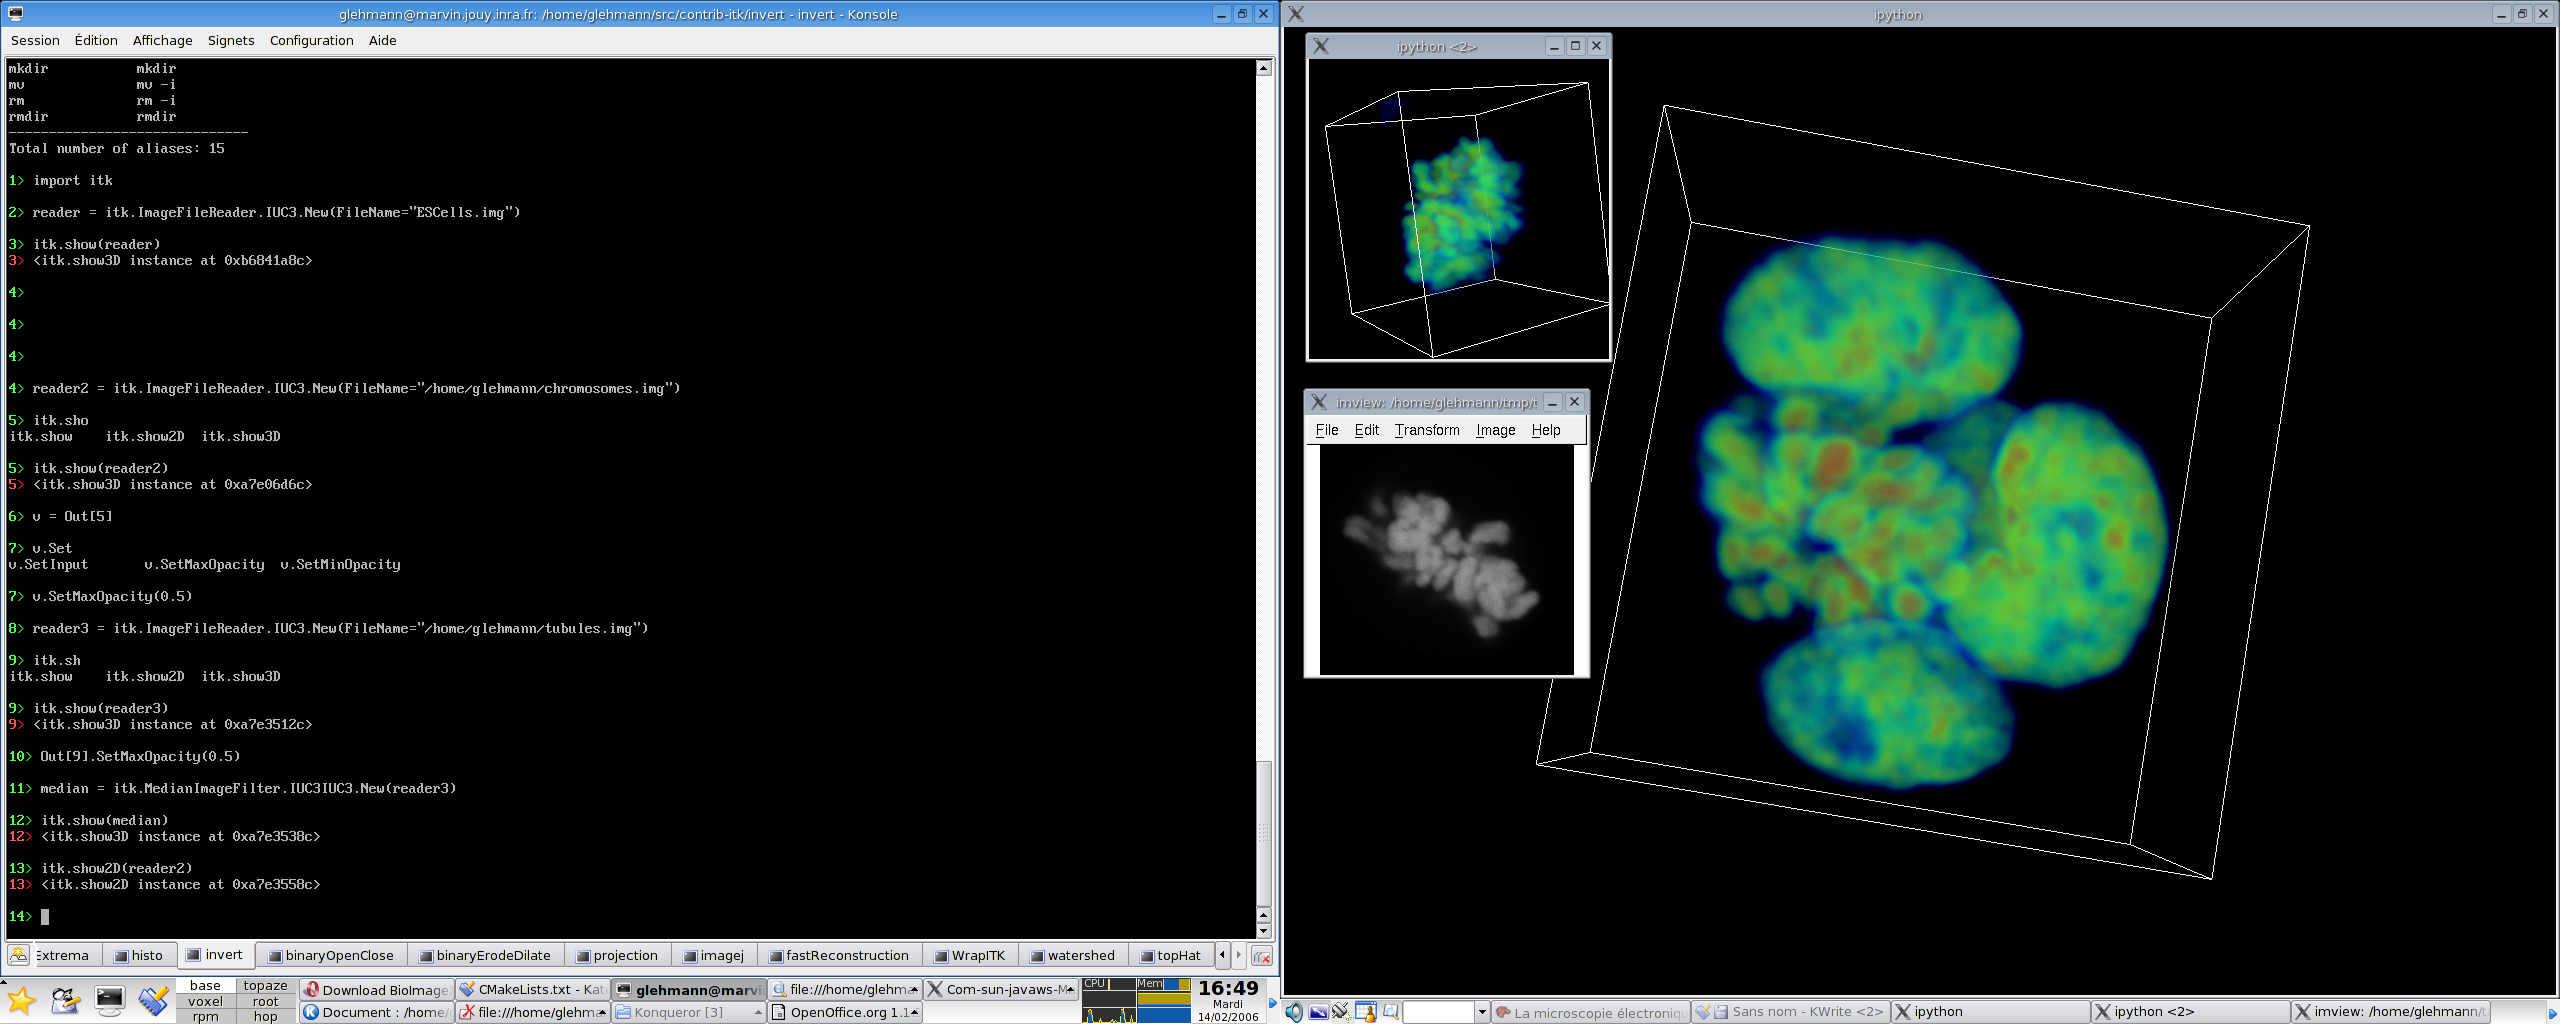
\includegraphics[scale=0.18]{capture1}
\caption{A screenshot of WrapITK in action with python.\label{screenshot}}
\end{figure}

  \item \verb$itk.strel(d, s)$ is used to create a binary ball structuring of dimension
\verb$d$ and size \verb$s$. Structuring element support is quite bad currently in WrapITK
and should change in the future. Using \verb$itk.strel$ rather than creating a
\verb$BinaryBallStructuringElement$ directly is recommended to have backward compatibility
when the structuring element type changes.

  \item \verb$itk.auto_progress(b)$ is used to automatically add a progress report
to all the newly created filters. \verb$b$ must be \verb$True$ or \verb$False$. If
\verb$b$ is true, something like
\begin{verbatim}
9> median.Update()
itkMedianImageFilterIF2IF2: 0.109990
\end{verbatim}
is displayed on the standard output.
While prototyping, it is a convenient way for the user to know if
the execution time will be short or if he can do something more useful
\footnote{like having a cup of tea} than waiting for the filter to complete.

\verb$itk.auto_progress(True)$ also sets an import callback which show the module name when
the module are imported.

  \item \verb$itk.class_(object)$ returns the class of an object. The \verb$__class__$
attribute is often not what the user wants with ITK. \verb$itk.class_$ is a convenience
function to get the class of an ITK object.

Note that it is called \verb$class_$ and not \verb$class$, because \verb$class$ is a
reserved word in python.

Example:
\begin{verbatim}
10> median.__class__
10> <class 'itkMedianImageFilter.itkMedianImageFilterIF2IF2_PointerPtr'>

11> itk.class_(median)
11> <class 'itkMedianImageFilter.itkMedianImageFilterIF2IF2'>
\end{verbatim}

  \item \verb$itk.echo(object, file)$ is a convenience function to call the \verb$Print()$
method of an ITK object without the need to pass a \verb$StringStream$ object.
This function is less useful with the optional patches: the \verb$__str__()$
method does a very similar job with better integration with python.

Example:

\begin{verbatim}
12> itk.echo(median)
MedianImageFilter (0x82c5b68)
  RTTI typeinfo:   itk::MedianImageFilter<itk::Image<unsigned char, 3u>, itk::Image<unsigned char, 3u> >
  Reference Count: 1
  Modified Time: 10
  Debug: Off
  Observers:
    none
  Number Of Required Inputs: 1
  Number Of Required Outputs: 1
  Number Of Threads: 2
  ReleaseDataFlag: Off
  ReleaseDataBeforeUpdateFlag: Off
  No Inputs
  Output 0: (0x875da68)
  AbortGenerateData: Off
  Progress: 0
  Multithreader:
    RTTI typeinfo:   itk::MultiThreader
    Reference Count: 1
    Modified Time: 2
    Debug: Off
    Observers:
      none
    Thread Count: 2
    Global Maximum Number Of Threads: 0
  Radius: [1, 1, 1]
\end{verbatim}


  \item \verb$itk.pipeline$ class let the developer easily create
a custom pipeline which can then be manipulated as a pure ITK filter.
It provides several methods:
\begin{itemize}
  \item \verb$__init__( self, input=None )$ is the constructor of the pipeline.
The input of the pipeline can be passed as parameter.

  \item \verb$connect( self, filter )$ connect a new filter to the pipeline.
The output of the last filter in the pipeline will be set as the input of the filter
passed as a parameter, and the filter passed as a parameter will be added to the filter
list.

  \item \verb$append( self, filter )$ add a filter to the pipeline's filters list,
but don't connect it. The connection must be done by the user. This method is likely
to be used with filters with several inputs.

  \item \verb$clear( self )$  clear the filter list.

  \item \verb$GetOutput( self )$ return the output of the last filter in the pipeline.
If another output is needed, use \verb$pipeline[-1].GetAnotherOutput()$ instead of
this method, or subclass pipeline to implement another \verb$GetOutput()$ method.

  \item \verb$SetInput( self, input )$ set the input of the first filter in the
pipeline. If another input is needed, use \verb$pipeline[0].SetAnotherIntput()$ instead of
this method, or subclass pipeline to implement another \verb$SetIntput()$ method.

  \item \verb$GetInput( self )$ return the input of the last filter in the pipeline.
If another input is needed, use \verb$pipeline[0].GetAnotherInput()$ instead of
this method, or subclass the pipeline to implement another \verb$GetInput()$ method.

  \item \verb$Update( self )$ update the pipeline by calling \verb$Update()$ method
on the last filter in the pipeline.

  \item \verb$__getitem__( self, i )$ and \verb$__len__( self )$ provide the common
python list manipulation interface to the pipeline object.

\end{itemize}

Example:
ITK's current implementation of morphological dilation, erosion, opening and closing
can be very inefficient with large structuring elements. Also, WrapITK only gives
access to ball structuring element. The following class illustrates the use of the
\verb$itk.pipeline$ class to implement an efficient opening in 3 dimensions with
a box structuring element. We take advantage of structuring element decomposition:
a dilation (or erosion) by a box can be more efficiently computed by perfoming
3 dilations (or erosion) with line structuring element oriented on each dimension.
The \verb$itk.pipeline$ encapsulates the 6 filters needed to perform the efficient
opening, and takes care of setting the structuring elements for all the internal
filters in the \verb$SetKernel(self, x,y,z)$, according to the size wanted by the
user.

\begin{verbatim}
class mkOpeningPipe (itk.pipeline):
  def __init__(self, Input, x=1, y=1, z=1):
    im = itk.image(Input)
    itk.pipeline.__init__(self, im)
    KernelType = itk.class_(itk.strel(3, 0))
    InType = itk.class_(im)
    self.connect(itk.GrayscaleErodeImageFilter[InType, InType, KernelType].New())
    self.connect(itk.GrayscaleErodeImageFilter[InType, InType, KernelType].New())
    self.connect(itk.GrayscaleErodeImageFilter[InType, InType, KernelType].New())
    self.connect(itk.GrayscaleDilateImageFilter[InType, InType, KernelType].New())
    self.connect(itk.GrayscaleDilateImageFilter[InType, InType, KernelType].New())
    self.connect(itk.GrayscaleDilateImageFilter[InType, InType, KernelType].New())
    self.SetKernel(x,y,z)

  def SetKernel(self, x,y,z):
    self[0].SetKernel(itk.strel(3, (x,0,0)))
    self[1].SetKernel(itk.strel(3, (0,y,0)))
    self[2].SetKernel(itk.strel(3, (0,0,z)))
    self[3].SetKernel(itk.strel(3, (x,0,0)))
    self[4].SetKernel(itk.strel(3, (0,y,0)))
    self[5].SetKernel(itk.strel(3, (0,0,z)))
\end{verbatim}

The \verb$mkOpeningPipe$ object can be used as a standard ITK filter:

\begin{verbatim}
reader = itk.ImageFileReader.IUC3.New(FileName='image.tif')
opening = mkOpeningPipe(reader)
ws = itk.MorphologicalWatershedImageFilter.IUC3IUC3.New(opening)
itk.write(ws, "result.tif")
\end{verbatim}

\end{itemize}

     \subsection{Advanced Features}

As an extra bonus, it is possible to view the doxygen documentation for each
class as the python docstring. This string is available as:
\small \begin{verbatim}
print itk.Image.__doc__
\end{verbatim} \normalsize
or even better (if you use iPython)
\small \begin{verbatim}
itk.Image?
\end{verbatim} \normalsize

Several steps are necessary to obtain this nirvana, however. First, when
configuring the build in ccmake, you must set \verb$DOXYGEN_MAN_PATH$ to some directory
where man pages for the ITK classes will be created. Then, after the build, you
must run \verb$make_doxygen_config.py$ from within the \verb$Python$ directory in the build
directory, to collect information about the wrapped classes and create a doxygen
configuration file to make these man pages. Finally, run doxygen with that
configuration file. After these three simple steps, class docstrings will
contain the man page information. Note that this is limited to systems which
support the python \verb$commands$ module, and which have \verb$groff$ in the path. This
basically means anything but windows \cite{WindowsWebSite} will work. (Cygwin should work too.)

In addition (as mentioned above), WrapITK by default ensures that no bare
pointers are ever returned to python: instead, reference-counting \verb$SmartPointer$s
are used. However, there may be times when extracting a bare pointer or creating
a new \verb$SmartPointer$ is necessary. To get a bare pointer from a smart pointer, use
the \verb$GetPointer()$ method, as in ITK proper. To create a new smart pointer, the
\verb$SmartPointer$ template proxy class can be used just as above:
\small \begin{verbatim}
smartPtr = itk.SmartPointer[itk.Image[itk.US, 2]](image.GetPointer())
\end{verbatim} \normalsize
or just
\small \begin{verbatim}
smartPtr = itk.SmartPointer[image](image.GetPointer())
\end{verbatim} \normalsize

WrapITK modules can take very long to import. The \verb$itkConfig$ module defines
a \verb$ImportCallback$ method which will be called when each sub module is
imported in the import process. \verb$ImportCallback$ can be customized to report the
progress status of the import process. It must be a function that can take
the name of the library being imported as a parameter. Here is an example of a very
basic callback function which displays the name of the submodule being imported on
the standard error output.
\small \begin{verbatim}
import sys, itkConfig
def stderr_callback(name, progress):
  if progress == 0:
    print >> sys.stderr, "Loading %s..." % name,
  if progress == 1:
    print >> sys.stderr, "done"
itkConfig.ImportCallback = stderr_callback
import itk
\end{verbatim} \normalsize

\verb$progress$ takes only the values $0$ and $1$, but may take values between $0$ and $1$
in the future.

It must be noted that using \verb$import itk$ loads only python code, and doesn't load
any C++ compiled code. This feature is called {\em lazy loading}. It implies some specific
behaviors:
\begin{itemize}
 \item \verb$import itk$ is done in a very short time
 \item a compiled module is loaded only when a class in that module is used. Thus,
when a python program is run, only the revelant modules are loaded in memory
 \item using a class in a program can block the program (for a short time). The user
can choose to load the entire library at once with the command \verb$itk.force_load()$.
\end{itemize}

     \subsection{Full python script examples}

This script is the exact transcription to python of the C++ example
which can be found at Examples/Filtering/GradientMagnitudeRecursiveGaussianImageFilter.cxx
in the ITK source tree. More information about the filters used can be found in
the ITK Software Guide \cite{ITKSoftwareGuide}, section 6.4.2.

\small \begin{verbatim}
import itk
from sys import argv

InputPixelType = itk.F
OutputPixelType = itk.F

InputImageType = itk.Image[InputPixelType, 2]
OutputImageType = itk.Image[OutputPixelType, 2]

reader = itk.ImageFileReader[InputImageType].New( FileName=argv[1] )

filter = itk.GradientMagnitudeRecursiveGaussianImageFilter[InputImageType, OutputImageType].New(
                     reader,
                     Sigma=float(argv[3]) )
filter.Update();

WritePixelType = itk.UC
WriteImageType = itk.Image[WritePixelType, 2]

rescaler = itk.RescaleIntensityImageFilter[OutputImageType, WriteImageType].New( filter,
                     OutputMinimum=0,
                     OutputMaximum=255 )

writer = itk.ImageFileWriter[WriteImageType].New( rescaler, FileName=argv[2] )

writer.Update();
\end{verbatim} \normalsize

More examples can be found in the directory \verb$Python/Tests$.

    \section{TCL usage}

Some examples are available in \verb$Tcl/Tests$ directory.

Write me.

    \section{Java usage}

Some examples are available in \verb$Java/Tests$ directory.

Write me.

\newpage
\part{Developer guide}

What follows is a brief description of how the WrapITK build system works, how
it can be extended, and how to write external projects.

  \section{WrapITK description}

     \subsection{Creating a CMakeLists.txt file for a wrapper library}
Each WrapITK sub-library (e.g. \verb$Base$, or \verb$SpatialObject$) lives in a
sub-directory of the WrapITK project (within the \verb$Modules$ directory) with a
\verb$CMakeLists.txt$ file that describes how that library and its language support files
(e.g. python template definitions) is to be created. Moreover, any external
project will need a similar file to describe how to create that library.

See \verb$SampleCMakeLists.txt$ in this directory for a description of each macro and
option that can appear in such a file. What follows is the usual set of commands
that will appear:

\small \begin{verbatim}
BEGIN_WRAPPER_LIBRARY("MySpatialObjectExtensions")
SET(WRAPPER_LIBRARY_DEPENDS SpatialObject Base)
SET(WRAPPER_LIBRARY_LINK_LIBRARIES ITKCommon)
WRAPPER_LIBRARY_CREATE_WRAP_FILES()
WRAPPER_LIBRARY_CREATE_LIBRARY()
\end{verbatim} \normalsize

\begin{itemize}
  \item \verb$BEGIN_WRAPPER_LIBRARY()$ sets up the environment to wrap a set of classes into a
library with a given name. This macro is defined in \verb$ConfigureWrapping.cmake$.
\verb$WRAPPER_LIBRARY_DEPENDS$ stores the list of WrapITK libraries on which the
current library depends (e.g. which libraries wrap classes like \verb$Image$ or
\verb$SpatialObject$, that are going to be used in the current library). Every project
should at least depend on \verb$Base$.

  \item \verb$WRAPPER_LIBRARY_LINK_LIBRARIES$ stores a set of other libraries to add at link
time. These can be 3rd party libraries that you will use (be sure to properly set
\verb$LINK_DIRECTORIES$ in this case), or more commonly, the ITK libraries that need to
be linked in, like \verb$ITKCommon$, \verb$ITKIO$, etc.

  \item \verb$WRAPPER_LIBRARY_CREATE_WRAP_FILES()$ scans all of the \verb$wrap_XXX.cmake$ files in the
current directory and uses the directives within to create CableSwig input files
for these classes. Information about template instantiations is also recorded
for the language support files that are created next. This macro is defined in
\verb$CreateCableSwigInputs.cmake$, and calls language support macros from
\verb$CreateLanguageSupport.cmake$.

  \item Finally, \verb$WRAPPER_LIBRARY_CREATE_LIBRARY()$ creates rules to parse the CableSwig
inputs and compile a wrapper library. This macro also causes various language
support files to be created (currently only python) which makes it easy to load
that library in python, and which knows about the template instances defined.
This macro is defined in \verb$CreateWrapperLibrary.cmake$, and calls language support
macros from \verb$CreateLanguageSupport.cmake$.
\end{itemize}


     \subsection{Creating wrap\_XXX.cmake files to wrap classes}

A \verb$wrap_XXX.cmake$ file defines a group of classes and/or template instantiations
to be wrapped. Often one such file is defined for each class wrapped, but this
is not strictly necessary.

Within such a file, directives are issued to wrap classes and particular
template instances.

WrapITK define several macros and variables designed to:
\begin{itemize}
  \item make creation of wrappers easy. The syntax is simple enough start quickly.
  \item make the choice of template arguments explicit. It should be easy to understand
the idea of the author of a wrapper by reading the file.
  \item support mostly transparently the dimensions and types chosen by the user.
\end{itemize}

     \subsubsection{A simple example: MedianImageFilter}

The most common case should be to create a new wrapper for a simple image filter, like
\verb$MedianImageFilter$. Let's see that example in detail.

Here is the \verb$BasicFiltersB/wrap_itkMedianImageFilter.cmake$ file:

\small \begin{verbatim}
WRAP_CLASS("itk::MedianImageFilter" POINTER)
  WRAP_IMAGE_FILTER_USIGN_INT(2)
  WRAP_IMAGE_FILTER_SIGN_INT(2)
  WRAP_IMAGE_FILTER_REAL(2)
END_WRAP_CLASS()
\end{verbatim} \normalsize

The file contains a \verb$WRAP_CLASS$ - \verb$END_WRAP_CLASS$ block, which itself contains
some \verb$WRAP_IMAGE_FILTER_*$ macros. \verb$WRAP_CLASS("itk::MedianImageFilter" POINTER)$
begins the wrapping of the \verb$itk::MedianImageFilter$ templated class. The name of the class
must be fully qualified. The option \verb$POINTER$ indicates that the object of the class can be
manipulated with a \verb$SmartPointer$, and that the \verb$SmartPointer$ specialization for
the class \verb$itk::MedianImageFilter$ must be created.

Then, several \verb$WRAP_IMAGE_FILTER_*$ macros are called. They are convenient macro to
create wrapper for classes which take only image types as template arguments. The parameter,
here \verb$2$, give the number of required template arguments. The two image types used as
template parameter are the same.

     \subsubsection{WrapITK predifined lists}

The main task of the developer is to define which template parameters are valid for a given
templated class, and interesting for the user. He also have to take care about
instantiating some templated classes according to the options selected by the user.

With WrapITK, the developer don't have to declare that a class is instantiated with the template parameters
\verb$unsigned char$, \verb$unsigned short$, and \verb$unsigned long$, but rather declares that the
templated classe can be instantiated with all the unsigned integer types choosed by the user.
To do that, WrapITK provides some already defined list which are grouping the types chosen by
the user. Those lists can be used by the developer to create a wrappers but must
{\em never} be modified.

\begin{itemize}
  \item \verb$WRAP_ITK_DIMS$ contains all the dimensions selected by the user.

  \item \verb$WRAP_ITK_USIGN_INT$ contains all unsigned integer types selected by the user.

  \item \verb$WRAP_ITK_SIGN_INT$ contains all signed integer types selected by the user.

  \item \verb$WRAP_ITK_INT$ contains all signed and unsigned integral types
selected by the user.

  \item \verb$WRAP_ITK_REAL$ contains all the real types selected by the user.

  \item \verb$WRAP_ITK_SCALAR$ contains all the scalar types selected by the user.

  \item \verb$WRAP_ITK_RGB$ contains all the \verb$RGB$ types selected by the user.

  \item \verb$WRAP_ITK_VECTOR_REAL$ contains all the \verb$Vector$ types selected
by the user.

  \item \verb$WRAP_ITK_COV_VECTOR_REAL$ contains all the \verb$CovariantVector$ types selected
by the user.

  \item \verb$WRAP_ITK_VECTOR$ contains all the \verb$Vector$ and
\verb$CovariantVector$ types selected by the user.

  \item \verb$WRAP_ITK_ALL_TYPES$ contains all the types selected by the user.

  \item \verb$SMALLER_THAN_D$ contains all the types "smaller" than \verb$double$
selected by the user. This variable is useful when a filter decrease the range
of pixel value, like \verb$BinaryThresholdImageFilter$.

  \item \verb$SMALLER_THAN_UL$ contains all the types "smaller" than \verb$unsigned long$
selected by the user.

  \item \verb$SMALLER_THAN_US$ contains all the types "smaller" than \verb$unsigned short$
selected by the user.

  \item \verb$SMALLER_THAN_SL$ contains all the types "smaller" than \verb$signed long$
selected by the user.

  \item \verb$SMALLER_THAN_SS$ contains all the types "smaller" than \verb$signed short$
selected by the user.

\end{itemize}


     \subsubsection{WrapITK predifined variables and naming consistency}

WrapITK defines some pairs of variables for each basic type the developer may have
to manipulate: the c++ type, and its template parameter name. The name of the type
is stored in \verb$ITKM_???$, and the c++ type in \verb$ITKT_???$.

For example, for \verb$unsigned char$, \verb$ITKM_UC$ and \verb$ITKT_UC$
are defined, with \verb|${ITKM_UC} = "UC"| and \verb|${ITKM_UC} = "unsigned char"|.

     \subsubsection{WrapITK macros}

All of the available directives are defined and documented
in \verb$CreateCableSwigInputs.cmake$. The basics are presented here:

\begin{itemize}
  \item \verb$WRAP_CLASS("fully_qualified::ClassName" [POINTER|POINTER_WITH_SUPERCLASS])$
causes a templated class to be wrapped. All namespaces must be included in the
class name, and note that no template instantiation is given. Template
instantiations are created with various \verb$WRAP$ directives, described below,
between invocations of \verb$WRAP_CLASS()$ and \verb$END_WRAP_CLASS()$.

\verb$WRAP_CLASS("itk::ImageFilter")$ issues an implicit call to \verb$WRAP_INCLUDE("itkImageFilter.h")$, so the header
for the wrapped class itself does not need to be manually included. To disable
this behavior, set \verb$WRAPPER_AUTO_INCLUDE_HEADERS$ to \verb$OFF$.

The final optional parameter to \verb$WRAP_CLASS$ is \verb$POINTER$ or
\verb$POINTER_WITH_SUPERCLASS$. If no options are passed, then the class is wrapped
as-is. If \verb$POINTER$ is passed, then the class and the typedef'd \verb$class::Pointer$
type is wrapped. (\verb$Class::Pointer$ had better be a \verb$SmartPointer$ instantiation, or
things won't work. This is always the case for ITK-style code.) If
\verb$POINTER_WITH_SUPERCLASS$ is provided, then \verb$class::Pointer$, \verb$class::Superclass$ and
\verb$class::Superclass::Pointer$ are all wrapped. (Again, this only works for
ITK-style code where the class has a typedef'd \verb$Superclass$, and the superclass
has \verb$Self$ and \verb$Pointer$ typedefs). \verb$POINTER_WITH_SUPERCLASS$ is especially
useful for wrapping classes whose superclasses depend on the template definitions of the given
filter. E.g. any of the functor image filters, which define totally different superclass
template parameters depending on which functor is used.

  \item \verb$END_WRAP_CLASS()$ -- end a block of template instantiations for a particular
class.

  \item \verb$WRAP_INCLUDE("header.h")$. By default, \verb$itkMedianImageFilter.h$ is included
when \verb$itk::MedianImageFilter$ is wrapped, and this behavior is usually
enough. If it not enough, this macro can be used to include some specific files.

  \item \verb$WRAPPER_AUTO_INCLUDE_HEADERS$. This variable is set to \verb$ON$ by default, but can
be set to \verb$OFF$ to disable the auto include feature. This feature should be used when several
classes to wrap come from the same header file.
\verb$WRAPPER_AUTO_INCLUDE_HEADERS$ is re-set to \verb$ON$ for each new \verb$wrap_xxx.cmake$ file.

  \item \verb$WRAP_TEMPLATE("mangled_suffix" "template parameters")$. When issued between \verb$WRAP_CLASS$
and \verb$END_WRAP_CLASS$, this command causes a particular template instantiation of
the current class to be wrapped. The parameter \verb$mangled_suffix$ is a suffix to
append to the class's name that uniquely identifies this particular template
instantiation, and "template parameters" are whatever should go between the \verb$< >$
template instantiation brackets. (Do not include the brackets.) If you are
wrapping a filter, there are simpler macros to use, which are defined at the
bottom of \verb$CreateCableSwigInputs$ and described below.

  \item \verb$WRAP_NON_TEMPLATE_CLASS("fully_qualified::ClassName" [POINTER|POINTER_WITH_SUPERCLASS])$.
Same as \verb$WRAP_CLASS$, but creates a wrapper
for a non-templated class. No \verb$END_WRAP_CLASS()$ is necessary after this macro
because there is no block of template instantiating commands to close.

\end{itemize}

WrapITK provides some macros to manipulate those list and uses them
to create the wrappers. Most of those macros are there to fill a lack
of features to manipulate lists in CMake, and should be replaced by
some CMake native commands in the future.

\begin{itemize}
  \item \verb$UNIQUE(var list)$ creates a new list called \verb$var$ composed of the same
elements as the ones in \verb$list$ without duplicates. This macro is useful to impose
a type even if it hasn't been selected by the user. The following line for example, from
\verb$Modules/IO/wrap_itkImageFileReader.cmake$, forces the unsigned char type to be
wrapped:

\small \begin{verbatim}
  UNIQUE(image_types "UC;${WRAP_ITK_ALL_TYPES}")
\end{verbatim} \normalsize

  \item \verb$SORT(var list)$ creates a new list called \verb$var$ which contains the
same elements as \verb$list$, sorted lexicographically

  \item \verb$INTERSECTION(var list1 list2)$ creates a new list called \verb$var$ which
is the intersection of lists \verb$list1$ and \verb$list2$

  \item \verb$REMOVE(var list1 list2)$ removes elements in \verb$list2$ from \verb$list1$
and store the result in \verb$var$

  \item \verb$INCREMENT(var number)$ increments \verb$number$ by one and stores the result
in \verb$var$

  \item \verb$DECREMENT(var number)$ decrement \verb$number$ by one an store the result
in \verb$var$

  \item \verb$FILTER_DIMS(var dimension_condition)$ processes a \verb$dimension_condition$
and returns a list of the dimensions that (a) meet the condition, and (b) were selected
to be wrapped. Recall that the condition is either a CMake list of dimensions, or a
string of the form "n+" where n is a number.

\end{itemize}


Some convenient macros are available to wrap image filters.

These macros often take an optional second parameter which is a "dimensionality
condition" to restrict the dimensions that the filter will be instantiated
for. The condition can either be a single number indicating the one dimension
allowed, a list of dimensions that are allowed (either as a single \verb$-$delimited
string or just a set of separate parameters), or something of the form \verb$n+$
(where \verb$n$ is a number) indicating that instantiations are allowed for dimension
n and above.


\begin{itemize}

  \item \verb$WRAP_IMAGE_FILTER_type(size)$ . \verb$type$ can be one of:
  \begin{itemize}
    \item \verb$USIGN_INT$ to select all the image types with unsigned integral
pixel types selected by the user
    \item \verb$SIGN_INT$ to select all the image types with signed integral
pixel types selected by the user
    \item \verb$INT$ to select all the image types with signed and unsigned integral
pixel types selected by the user
    \item \verb$REAL$ to select all the image types with real pixel types selected by the user
    \item \verb$VECTOR_REAL$ to select all the image types with \verb$Vector$
pixel types selected by the user
    \item \verb$COV_VECTOR_REAL$ to select all the image types with \verb$CovariantVector$
pixel types selected by the user
    \item \verb$RGB$ to select all the image types with \verb$RGBPixel$
pixel types selected by the user
    \item \verb$SCALAR$ to select all the image types with scalar pixel types selected by the user
    \item \verb$VECTOR$ to select all the image types with \verb$Vector$ and \verb$CovariantVector$
pixel types selected by the user
    \item \verb$ALL_TYPES$ to select all the image types selected by the user.
  \end{itemize}

 This macro creates a template instantiation with \verb$size$
\verb$itk::Image$ parameters of the given pixel type. So if you are wrapping a filter
which should take two images with integral pixel types, write \verb$WRAP_IMAGE_FILTER_USIGN_INT(2)$. The
specific integral data type(s) (\verb$char$, \verb$long$, or \verb$short$ in the \verb$WRAP_IMAGE_FILTER_USIGN_INT$ case) will
be determined by the user-selected build parameters (e.g. \verb$WRAP_long$, and
\verb$WRAP_short$).

  \item \verb$WRAP_IMAGE_FILTER(param_types param_count)$ is a more general
macro for wrapping image filters that need one or more image parameters of the
same type. The first parameter to this macro is a list of image pixel types for
which filter instantiations should be created. The second is a \verb$param_count$
parameter which controls how many image template parameters are created. The
optional third parameter is a dimensionality condition.

E.g. \verb@WRAP_IMAGE_FILTER("${WRAP_ITK_ALL}" 2)@ will create template instantiations
of the filter for every pixel type that the user has selected.


  \item \verb$WRAP_IMAGE_FILTER_TYPES()$. Creates template instantiations of the
current image filter for all the dimensions selected by the user (or dimensions
selected by the user that meet the optional dimensionality condition). This
macro takes a variable number of arguments, which should correspond to the image
pixel types of the images in the filter's template parameter list. The optional
dimensionality condition should be placed as the last parameter.

  \item \verb$WRAP_IMAGE_FILTER_COMBINATIONS()$ takes a variable number of
parameters. Each parameter is a list of image pixel types. Filter instantiations
are created for every combination of different pixel types in different
parameters. A dimensionality condition may be optionally specified as the first
parameter. E.g. \verb$WRAP_IMAGE_FILTER_COMBINATIONS("UC;US" "UC;US")$ will
create: \verb$filter<itk::Image<unsigned char, d>, itk::Image<unsigned char, d> >$,
\verb$filter<itk::Image<unsigned char, d>, itk::Image<unsigned short, d> >$,
\verb$filter<itk::Image<unsigned short, d>, itk::Image<unsigned char, d> >$, and
\verb$filter<itk::Image<unsigned short, d>, itk::Image<unsigned short, d> >$
where \verb$d $is the image dimension, for each selected image dimension.

%   \item \verb$WRAP_type_DIMS(size dims)$ (with \verb$type$ as above) -- Wrap a filter for certain
% dimensions only. Dims should be either a semicolon-separated list of valid
% dimensions, or something of the form \verb$'3+'$ to specify that the filter can be
% instantiated only for three- and higher-dimensional images. Note that if the
% user has not selected to wrap a given dimension at build time, a filter wrapped
% with \verb$WRAP_type_DIMS$ will not be instantiated: the final dimensions wrapped are
% the {/em intersection} of the user-selected dimensions and the valid dimensions
% declared with \verb$WRAP_type_DIMS$.

\end{itemize}


  \section{Extending or customizing WrapITK}

To minimize build times and library size, it is possible to manually prevent
various classes from being wrapped. WrapITK is divided into several
sub-libraries, each with a sub-directory: \verb$Algorithms$, \verb$BasicFilters[ABC]$,
\verb$Common[AB]$, \verb$IO$, \verb$Numerics$, \verb$SpatialObject$, and \verb$VXLNumerics$. Within these
directories are sets or \verb$wrap_XXX.cmake$ files, where \verb$XXX$ is the name of the class
(or set of classes) to be wrapped. To prevent one of these classes from being
wrapped, simply rename the file to anything that does {\em not} start with \verb$wrap_$ and
end with cmake. (E.g. append \verb$.notwrapped$ to the name.) (This is probably
unsafe to do in the \verb$Common$, \verb$Numerics$, or \verb$IO$ directories.)

To add classes to be wrapped, it is recommended that you create a simple
{\em External Project} described below. If this is out of the question, you could
create additional \verb$wrap_XXX.cmake$ files in the appropriate directory. (Read on
for instructions as to what to put in these files.)


  \section{External projects}

    \subsection{Why external projects?}

External projects let the developer access some custom class with the target languages
and is a powerful way to extend WrapITK, test new wrapper, wrap more types, etc.
A nice side effect of wrappers, for contributions\footnote{A nice template for
contributions to the Insight Journal \cite{InsightJournalWebSite} which include the
template code to build wrappers is available at
\url{http://voxel.jouy.inra.fr/darcs/contrib-itk/template/}. Just use the command
{\em darcs get http://voxel.jouy.inra.fr/darcs/contrib-itk/template/ contribName}
and edit the project name in the {\em CMakeLists.txt} file to
begin your new contribution.}, for example, to build {\em all}
the methods of the wrapped classes, and so to be sure everything builds as it should
\footnote{We have found and fixed  a number of bugs in ITK while adding
more classes to WrapITK}.
In WrapITK, we used them to avoid managing switches if some dependencies are not
found: the project must find its dependencies or fail.

External projects are not yet supported for Tcl and Java. See \ref{section:contribute}
to contribute external project support for those languages.

    \subsection{Building}
To build an external project, first ensure that WrapITK has been properly built.
Then use \verb$ccmake$ to configure a build directory for the external project. If
WrapITK has not been installed, you will have to manually enter the path to the
WrapITK build directory.

By default, the build options are the same than the one used for building WrapITK,
but can be modified in the advanced options.

    \subsection{Usage}
Once an external project has been built, it can be tested directly from the
build tree. Start python in the external project build directory's Python
subdirectory, and run the command \verb$import ProjectConfig$ (or
\verb$import ProjectConfig-[Debug|Release|...]$ if you are using an IDE, depending on which
build configuration was set from the IDE). This command sets up the search paths
properly so that WrapITK and the newly-created library files can be found. Then
type \verb$import ...$ (where \verb$...$ is replaced with the name of the external
project; e.g. \verb$import BufferConversion$), and use the project.

    \subsection{Installation}
Simply type \verb$make install$ (or run your IDE's install step) to install the
external project into the WrapITK tree (provided WrapITK has already been
installed). Now the external project can be used just like any of the other
WrapITK libraries, and it will be imported into the \verb$itk$ namespace when the
\verb$import itk$ command is issued from Python.

    \subsection{Top-level CMakeLists for external projects}
In addition to having a set of \verb$wrap_XXX.cmake$ files and the proper
commands to read in these files and create a library (all described above), an
external project's CMakeLists file needs at least one additional command to
start it out: \verb$FIND_PACKAGE(WrapITK REQUIRED)$.

This command will cause cmake to try to find the WrapITK build/install
directory. If WrapITK has been installed, this will work on the first try.
Otherwise, you will have to set (within ccmake, or in the CMakeLists if you
prefer) the variable \verb$WrapITK_DIR$ to contain the path to the WrapITK build
directory.

    \subsection{Examples}

In \verb$WrapITK/ExternalProjects$ there are several sample "External Projects" that
can be built to provide additional functionality to WrapITK and to serve as a
demonstration for how to create your own such projects. One project is an
ITK-VTK \cite{VtkWebSite} bridge, and the other is a Python class to allow conversion from
Numeric/Numarray/numpy \cite{NumericWebSite,NumarrayWebSite,NumpyWebSite} matrices to
ITK images (and vice-versa).

More examples can be found in the contributions to the Insight Journal
\cite{InsightJournalWebSite}, or directly at \url{http://voxel.jouy.inra.fr/darcs/contrib-itk/}.

    \subsection{BufferConversion: an example of extension for one language}

This project is a python only project. It requires you to have Numeric, Numarray or numpy installed
on your system, and will let the user convert ITK images to python matrices, and python matrices
to ITK images. It thus provide a bridge between ITK and other great python tools like SciPy
\ref{SciPyWebSite} (and a lot of others).

Once installed, the function are directly available in the \verb$itk$ module - there is nothing
special to import. A \verb$PyBuffer$ template let you choose the type to convert, exactly
like with the ITK classes. You can then use the \verb$GetArrayFromImage()$ and
\verb$GetImageFromArray()$ method to convert an array to an ITK image, and an
ITK image to an array respectively. There is no need to instantiate a \verb$PyBuffer$ object: the methods
are \verb$static$.

\begin{verbatim}
1> import itk

2> reader = itk.ImageFileReader.IUS2.New(FileName='cthead1.png')

3> array = itk.PyBuffer.IUS2.GetArrayFromImage(reader.GetOutput())

4> array
4>
array([[0, 0, 0, ..., 0, 0, 0],
       [0, 0, 0, ..., 0, 0, 0],
       [0, 0, 0, ..., 0, 0, 0],
       ...,
       [0, 0, 0, ..., 0, 0, 0],
       [0, 0, 0, ..., 0, 0, 0],
       [0, 0, 0, ..., 0, 0, 0]], type=UInt16)

5> image = itk.PyBuffer.IUS2.GetImageFromArray(array)

6> image
6> <C itk::SmartPointer<(itk::Image<(unsigned short,2)>)> instance at _50684208_p_itk__SmartPointerTitk__ImageTunsigned_short_2_t_t>
\end{verbatim}

Because PyBuffer is a python only external project, its directory structure is very
simple - there is no subdirectory. This external project should be used as an example
for all the languages specific external projects.

    \subsection{ItkVtkGlue: an example of extension for all languages, including C++}

ItkVtkGlue wraps the classes used to convert data from ITK to VTK \cite{VtkWebSite} and from VTK to ITK.
Those classes comes from the InsightApplications \cite{ITKWebSite}, and make the conversion
as simple in python as in C++. It has been tested with VTK 5.0.0.

With python lazy loading, the classes are not loaded by default, and thus avoid
loading the entire vtk code in memory. The classes are directly available in the
\verb$itk$ module, and the underlying code is loaded only when those classes are used.

Example:
\begin{verbatim}
1> import itk

2> reader = itk.ImageFileReader.IUC3.New()

3> converter = itk.ImageToVTKImageFilter.IUC3.New(reader)

4> converter.GetOutput()
4> <libvtkFilteringPython.vtkImageData vtkobject at 0xb7675b60>
\end{verbatim}

The \verb$itk.show3D$ class uses the class \verb$ImageToVTKImageFilter$ to create the
volume rendering shown in Figure \ref{screenshot}.

This project provides new features for all the languages, including C++.
Its directory structure reflects this.

\begin{verbatim}
|-- CMakeLists.txt
|-- Wrapping
|   |-- CMakeLists.txt
|   |-- Python
|   |   |-- CMakeLists.txt
|   |   |-- Tests
|   |   |   |-- CMakeLists.txt
|   |   |   |-- CannyEdgeDetectionImageFilter.py
|   |   |   `-- simpleItkVtkPipeline.py
|   |   `-- itkvtk.py
|   |-- itkvtk.swg
|   |-- wrap_itkImageToVTKImageFilter.cmake
|   `-- wrap_itkVTKImageToImageFilter.cmake
|-- images
|   `-- cthead1.png
`-- src
    |-- itkImageToVTKImageFilter.h
    |-- itkImageToVTKImageFilter.txx
    |-- itkVTKImageToImageFilter.h
    `-- itkVTKImageToImageFilter.txx
\end{verbatim}

The C++ source files are in
directory src, while the files needed for WrapITK are in Wrapping.
The CMakeLists.txt file in the root of the project includes the
Wrapping sub directory only if the user ask for it with the option
BUILD\_WRAPPERS. Some python specific code can be found in Wrapping/Python
directory, and some python tests in Wrapping/Python/Tests.
The itkvtk.swg file contains the typemaps required to return vtk
objects.
The images directory contains the images used for the tests. Putting
the images in this directory rather than in the root of the project
prevents overriding the reference files during the test, which might occur if the build
is done in the source tree.
The project should also provide C++ tests - it is not done yet.


  \section{Extending language support and adding more languages}

Write me.

    \subsection{Generating target language code}

Write me.

    \subsection{typemaps}

Write me.

  \section{Contributing to WrapITK}
\label{section:contribute}

WrapITK is an open source project, so all contributions are welcome. Here are
some points which requires special attention:
\begin{itemize}
  \item Test it and report problem. That's the most important thing to do:
we need feedback to enhance WrapITK quality! Report all bugs you may find
to \url{http://voxel.jouy.inra.fr/roundup/wrapitk/} \cite{RoundupWebSite}.
  \item Work on tcl, java, and others. We are not tcl or java developers, and so
are not able to complete the work for those languages. Any help from tcl and
java expert would be highly appreciated. Also, there is no reason to be limited
to python, tcl and java, and WrapITK can be extended to other languages supported
by swig like perl \cite{PerlWebSite}, ruby \cite{RubyWebSite}, ocaml \cite{OcamlWebSite} and others.
  \item Add more classes. WrapITK adds many new classes compared to the current
wrapping system, but there is still a lot of work to do, especially to support more
filters dedicated to \verb$Vector$ pixels.
\end{itemize}

\verb$darcs$ \cite{DarcsWebSite} allows you to easily contribute to WrapITK, by sending
patches by email, while keeping credits for the work you have done.
Feel free to send patches; they will be tested and integrated in the project.

The basic commands to know are:
\begin{itemize}

  \item \verb$darcs get --partial http://voxel.jouy.inra.fr/darcs/contrib-itk/WrapITK/$
to get a copy of WrapITK repository.

  \item \verb$darcs whatsnew$ to display the changes you have made in
your copy of the repository.

  \item \verb$darcs record$ to record the changes you have made in your
copy of the repository. darcs will ask you to select some changes
to record. It is better to create one patch for each feature or bug
fix, rather than one big patch for all your current changes.

  \item \verb$darcs send$ to send the patches you have recorded with
\verb$darcs record$ by email. Please send your patches to the WrapITK bugtracker
(wrapitk-bugmaster@jouy.inra.fr\footnote{Note that you must have an account to
be able to send something to the bug tracker. Visit
\url{http://voxel.jouy.inra.fr/roundup/wrapitk/} to create one.}) so everyone
will be able to find it easily.

\end{itemize}

Read the {\em Getting started} section of the darcs manual \cite{DarcsWebSite}
for more information.

A web interface \cite{DarcswebWebSite} for the WrapITK's darcs
repository is available at \url{http://voxel.jouy.inra.fr/darcsweb/}.


\newpage
\part{Known bugs}
See \url{http://voxel.jouy.inra.fr/roundup/wrapitk/}.

\newpage
\part{Acknowledgments}
I thank Dr Pierre Adenot and all the {\em Embryon et Biotechnologie} team for their
patience during the long development time before getting the tool really usable.

We would like to thank Charl P. Botha for is help to debug WrapITK on the windows
platform, and for the patches he has contributed, as well as Richard Beare for
his early interest in using itk with python, for his useful feedback, and for
his work on buffer conversions in python.

We thank Andr\'e Bongers for his help debugging the java build on windows.

We thank Brad King for his assistance during the development process.

Finally, we thank the ITK developers for the great tool which is ITK, and for the
previous work done on the wrapping system - without it WrapITK would not exist.


\newpage
\part{Conclusion}

ITK is a great library, with the drawback of being nearly unusable for prototyping,
and having poor support for other languages than C++. WrapITK addresses those
issue and finally gives ITK a good support for python. Java and Tcl, while
not as complete as python, also benefit from the larger number of
wrapped classes, and of the increase of consistency in available types and names.



\newpage
\appendix



\bibliographystyle{plain}
\bibliography{Article,InsightJournal}
\nocite{ITKSoftwareGuide}

\end{document}
